\section{Results}

\subsection{Five minutes from scratch measures nothing}\label{sec:calibration}
Our first harness followed autoresearch exactly: each experiment trained a fresh model for five
minutes. On the M4 that is about 255 optimizer steps (4.2M tokens) for the 7.3M-parameter looped model.
Table~\ref{tab:calib} lists what we tried before giving up on this design. Every configuration left
reasoning at chance, including the easiest possible version of the task (zero hops: read a digit that
is stated earlier in the same line), a plain six-layer transformer, answer-only losses, a pure reasoning
stream with no text, and runs of up to 3,000 steps. An early arithmetic variant appeared to score 14--15\%,
but that was the digit prior: removing the bias brought it to 10\%.

\begin{table}[h]
\centering\small
\begin{tabular}{lrl}
\toprule
setup & steps & result \\
\midrule
arithmetic chains, $d{=}256$, 4 loops & 345 & chance \\
arithmetic chains, answer-only loss & 509 & chance \\
pointer chains, answer-only loss & 517 & chance \\
one hop only, answer-only loss & 316 & answer loss stuck at $\ln 10$ \\
dense variable tracking, hops 1--6, $d{=}384$ & 414 & chance \\
dense variable tracking, $d{=}256$, context 256 & 1,559 & chance \\
zero hops only, plain 6-layer transformer & 1,194 & chance \\
dense variable tracking, hops 0--6, LR $2{\times}10^{-3}$ & 2,980 & chance, unstable \\
\bottomrule
\end{tabular}
\caption{Calibration runs from scratch on the reasoning task (no text in the stream unless noted).
Chance is 10\%.}
\label{tab:calib}
\end{table}

Per-character losses showed why: local syntax was learned almost immediately (about 0 bits for
\texttt{=} and \texttt{;}), but the query letter cost about 4.6 bits (uniform over 26) and the answer
about 3.3 bits (uniform over 10). No retrieval circuit had formed. To rule out a bug we ran
multi-query associative recall~\citep{arora2024zoology} with 16 key--value pairs for 3,000 steps: our
block reached 22.9\%, an independently written minimal MLX transformer with learned positions,
LayerNorm and GELU reached 22.8\%, and our block at learning rate $3{\times}10^{-3}$ reached only 5.2\%.
The fused attention kernel matched a manual implementation to $6{\times}10^{-7}$. So the model was
correct; in-context retrieval simply emerges late, the familiar phase change of induction
heads~\citep{olsson2022context}, and higher learning rates delay it.

The fix is the two-stage protocol of \S\ref{sec:setup}. With continued training the looped base leaves
chance within the first \V{base-first-min} minutes (\V{base-first-hop1} at one hop;
Figure~\ref{fig:curves}). The lesson generalizes beyond this paper: an autoresearch budget has to be
long enough for the capability being measured to exist, or the agents will optimise noise. At laptop
scale, that means experiments on capabilities that emerge late should modify a trained model, not
train new ones.

\subsection{Looping versus conventional transformers at matched time}\label{sec:controls}
DRAFT

\begin{figure}[t]
\centering
\IfFileExists{figures/curves.pdf}{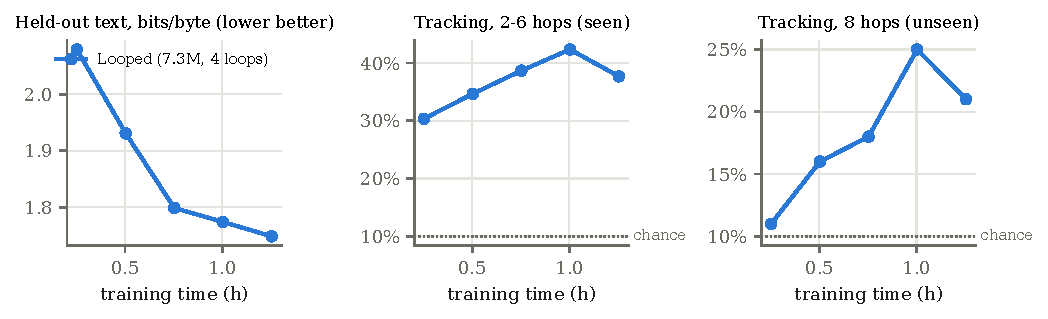
\includegraphics[width=\linewidth]{figures/curves.pdf}}{}
\caption{Training curves (quick evaluation, 100 problems per depth).}
\label{fig:curves}
\end{figure}

\subsection{The agent swarm}\label{sec:swarm}
DRAFT
